Now, relative standard deviation
$$\frac{\langle (2S)^2 \rangle}{N} = \frac{1}{\sqrt{N}}$$

For that lets define new variable $X = \frac{2S}{N}$, then
$$\rho(X) = \qty(\frac{N}{2\pi})^{\frac{1}{2}} e^{-\frac{NX^2}{2}}$$
\paragraph{Ergodic hypothesis}
For closed system ($B$, $E$, $N$, $V$ are constant) there is equal probability to acquire any of possible states. Such ctates are called \textbf{microcanonical ensemble}.

Example of exceptions:
\begin{center}
	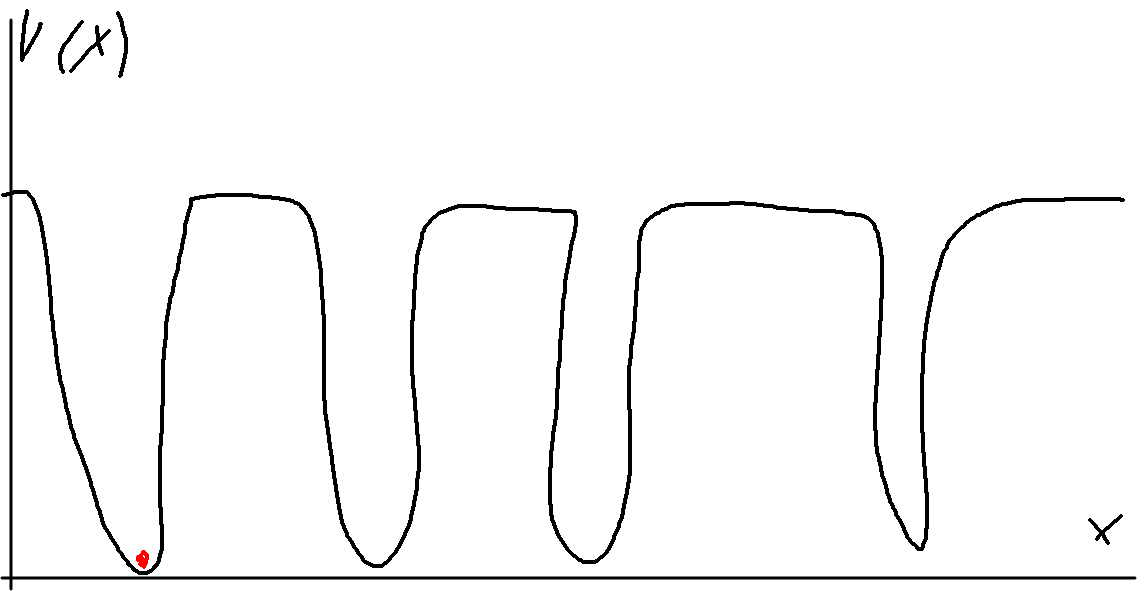
\includegraphics[width=\linewidth]{./lect4/pic1.png}
\end{center}
Particle can't get out of potential well though there are other well is could possible be into.

\paragraph{Meaning of ergodic hypothesis}
Suppose we have two closed Ising systems (with magnetic moments) and we connect them: one with $N_1=5$ and $2S_1=1$ and second with $N=10$ and $2S_2 = -2$.

Now, suppose we connected two systems to a single one.

If in each side nothing changes,
$$g^0_f = g_i = \frac{5!}{3!\cdot 2!} \cdot \frac{10!}{6!4!}$$

If one particle changes moment such that $2S_2 = 0$:
$$g^1_f = \frac{5!}{2!\cdot 3!} \cdot \frac{10!}{5!5!}$$
Note that $\frac{g_1^f}{g^0_f } = \frac{6}{5} > 1$.

If two particle changes moment such that $2S_2 = -2$:
$$g^2_f = \frac{5!}{1!\cdot 4!} \cdot \frac{10!}{6!3!}$$
Note that $\frac{g_1^f}{g^2_f } = \frac{6\cdot  \cdot 4}{ 5 \cdot 2 } > 1$.

Thus $g^1_f$ is most degenerated state, and the system will most of the time be on the most degenerated state. In big system, since variance of $X$ is $\frac{1}{\sqrt{N}}$, this state will observed almost always. I.e., there is flow from second box to the first one.

\paragraph{Example}
Now lets use Gaussian approximation. Then new degeneracy is
$g(N_1, S_1) \cdot g(N_2, S_2)$
and the condition is $S_1+S_2+S$. We also denote $N_1+N_2=N$. We are searching for a maximum of degeneracy under constrain.
$$g(N_1,N_2,S_1,S_2) = g_1(0)g_2(0) e^{-\frac{2S_1^2}{N_1}-\frac{2S_2^2}{N_2}}$$
Where $g_1(0)$, $g_2(0)$ are normalization constants, which doesn't affect optimization. Since $S_2 = S-S_1$:
$$g(N_1,N_2,S_1,S_2) = g_1(0)g_2(0) e^{-\frac{2S_1^2}{N_1}-\frac{2(S-S_1)^2}{N_2}}$$
We can optimize $\ln g$ instead, since, it's monotonous:
$$\ln g = C -\frac{2S_1^2}{N_1}-\frac{2(S-S_1)^2}{N_2} $$
$$\dv{\ln g}{S} =  -\frac{4S_1}{N_1}+\frac{4(S-S_1)}{N_2} = 0$$
$$N_1(S-S_1) - N_2 S_1= 0$$
$$N_1S - N S_1= 0$$
$$  S_1= \frac{N_1S}{N}$$
Thus
$$  S_2=  \frac{N_2S}{N}$$
How many states are in maximal degeneracy?

$$g(N_1,N_2,S_1,S_2) = g_1(0)g_2(0) e^{-\frac{2S^2}{N}}$$

Suppose we are looking at different state
$$\begin{cases}
S_1 = S_1^{max} + \delta\\
S_2 = S_2^{max} - \delta
\end{cases}$$
Then
\begin{align*}
g(N_1,N_2,S_1,S_2) = g_{max}(N_1,N_2,S_1,S_2) \cdot \exp\qty(-\frac{4S_1^{max} \delta}{N_1}-\frac{2\delta^2}{N_1}+\frac{4S_2^{max} \delta}{N_2}-\frac{2\delta^2}{N_2}) = g_{max}(N_1,N_2,S_1,S_2) \cdot \exp\qty(-\frac{2\delta^2}{N_1}-\frac{2\delta^2}{N_2})
\end{align*}
For example, if $N_1=N_2=10^{22}$  and $\delta = 10^{12}$, i.e., $\frac{\delta}{N_1} = 10^{-10}$, 

$$g(N_1,N_2,S_1,S_2) = g_{max}(N_1,N_2,S_1,S_2) \cdot e^{-400}$$